\documentclass{article}
\usepackage[utf8]{inputenc}
\usepackage[T1]{fontenc}
\usepackage{graphicx}
\usepackage{float}
\usepackage{amsmath}
\usepackage{booktabs}

\title{Project 2 Report -- Systems Biology}
\author{
    Martyna Pawlak 459438\\
    \and
    Aleksandra Pawłowska 459439
}
\date{19 May 2026}

\begin{document}

\begin{titlepage}
    \centering
    \vspace*{4cm}

    {\Huge \textbf{Project 2 Report -- Systems Biology} \par}

    \vspace{2cm}

    {\Large
    Martyna Pawlak 459438\par
    \vspace{0.5cm}
    Aleksandra Pawłowska\par
    }

    \vfill

    {\large 19 May 2026 \par}
\end{titlepage}

\section{Part A}

% =============================================================================
\subsection{Task A1}

\subsubsection{Brief methods summary}
The analysis of the effect of mutations on ERK signal dynamics was documented in
the \texttt{TaskA1\_MutationComparison.ipynb} notebook, which uses the
\texttt{compare\_spatiotemporal\_behavior.py} file from the
\texttt{spatiotemporal-continuation/scripts/} directory.
The analysis included five cell lines: wild type (WT) and the following mutants:
\texttt{AKT1\_E17K}, \texttt{PIK3CA\_E545K}, \texttt{PIK3CA\_H1047R}, and
\texttt{PTEN\_del}.
Standard analysis parameters were used: spatial radius (\texttt{spatial\_radius})
of 60, time window (\texttt{future\_window\_frames}) of 3, and signal column
\texttt{ERKKTR\_ratio}.
Mean relative risk values and statistical significance tests were calculated based
on data from the \texttt{block\_level\_summary.csv} file, allowing comparison of
value distributions between mutation groups and the wild type (WT).
Mean relative risk data (\texttt{mean\_relative\_risk}) were extracted from the
\texttt{group\_level\_summary.csv} file.
To verify the statistical significance of differences between WT and individual
mutants, Mann--Whitney U tests with Bonferroni correction for multiple comparisons
were performed.

\subsubsection{Key results}

The main result of the analysis is a comparative table and a bar chart
illustrating the differences in signal spread.

\begin{figure}[H]
    \centering
    \includegraphics[width=0.8\linewidth]{7fb6c24f-82eb-49cb-a13c-b88613fe1e12.png}
\end{figure}

\begin{figure}[H]
    \centering
    \includegraphics[width=0.8\linewidth]{tableka.png}
\end{figure}

\subsubsection{Interpretation}

The red dashed line in the chart ($RR = 1$) represents the absence of
spatiotemporal correlation.
Values above one indicate the existence of a signal transmission mechanism within
the cell population.
Statistical analysis revealed that the \texttt{PIK3CA\_H1047R} mutation showed a
relative risk value substantially higher than both the red reference line and the
WT group.
The remaining mutants also exhibited values above the red line, but they were
similar to or lower than the WT level.
This suggests that these mutations may paradoxically make signal propagation more
diffuse than in the wild type.

A key finding of the analysis was the dramatic increase in relative risk observed
for the \texttt{PIK3CA\_H1047R} mutation ($RR \approx 3.20$), indicating
exceptionally strong signaling coupling between neighboring cells.
The \texttt{PIK3CA\_H1047R} mutation is located within the kinase domain of the
PI3K protein, leading to constitutive and strong pathway activation.
As a consequence, cells become highly sensitive to signals originating from
neighboring cells.
Activation of one cell may therefore trigger a rapid chain reaction in adjacent
cells, substantially increasing both the range and intensity of signaling across
the population.
In contrast, the remaining mutations may induce weaker but chronic pathway
activation, potentially leading to cellular habituation to signaling stimuli.
As a result, cells respond less efficiently to neighboring-cell activation, making
signal transmission less efficient and more chaotic.

% =============================================================================
\subsection{Task A2}

\subsubsection{Research question}

Do different PI3K--AKT pathway mutations exhibit different spatiotemporal relay
timescales for ERK signal propagation?
Specifically, does the lag $\tau^*$ at which the Relative Risk $\mathrm{RR}(\tau)$
is maximised differ between wild-type cells and cells carrying oncogenic mutations?

\subsubsection{Methods}

For each cell--frame observation (cell $c$, frame $t$) we define:
\begin{itemize}
  \item \textbf{Exposure}: at least one spatial neighbour of cell $c$ shows a
        \emph{jump event} (a large upward signal change) at frame $t$.
  \item \textbf{Response at lag $\tau$}: cell $c$ itself shows a jump event at
        frame $t + \tau$.
\end{itemize}

A \emph{jump event} is defined as a frame-to-frame signal increase
$\Delta s \geq \theta$, where $\theta$ is the 90th percentile of all positive
signal differences within the block (data-driven, per-block threshold).
Spatial neighbours are cells within a Euclidean radius of 60 image-coordinate
units at the same frame, identified via a k-d tree.
The Relative Risk at lag $\tau$ is:

\begin{equation}
  \mathrm{RR}(\tau) =
  \frac{P(\text{focal cell jumps at } t+\tau \mid \text{neighbour jumped at } t)}
       {P(\text{focal cell jumps at } t+\tau \mid \text{no neighbour jumped at } t)}
\end{equation}

We evaluated $\tau \in \{0,1,2,3,4,5,6\}$ frames
($0, 5, 10, 15, 20, 25, 30$\,min at 5\,min/frame acquisition).
For each lag and mutation, raw counts were pooled across all
experiment--site blocks before computing $\mathrm{RR}(\tau)$, avoiding bias from
averaging ratios across blocks of different sizes.
Signal: \texttt{ERKKTR\_ratio}.

Three cell lines were selected: \textbf{WT} (baseline), \textbf{AKT1\_E17K}
(gain-of-function point mutation constitutively activating AKT1 independently of
PI3K), and \textbf{PTEN\_del} (loss of PTEN phosphatase, leading to chronically
elevated PIP3 and secondary AKT hyperactivation).
Both mutants converge on AKT hyperactivation through mechanistically distinct
nodes, making them informative for comparing ERK relay kinetics.
Blocks analysed: WT $n=24$, AKT1\_E17K $n=21$, PTEN\_del $n=27$.

\subsubsection{Key results}

\begin{figure}[H]
  \centering
  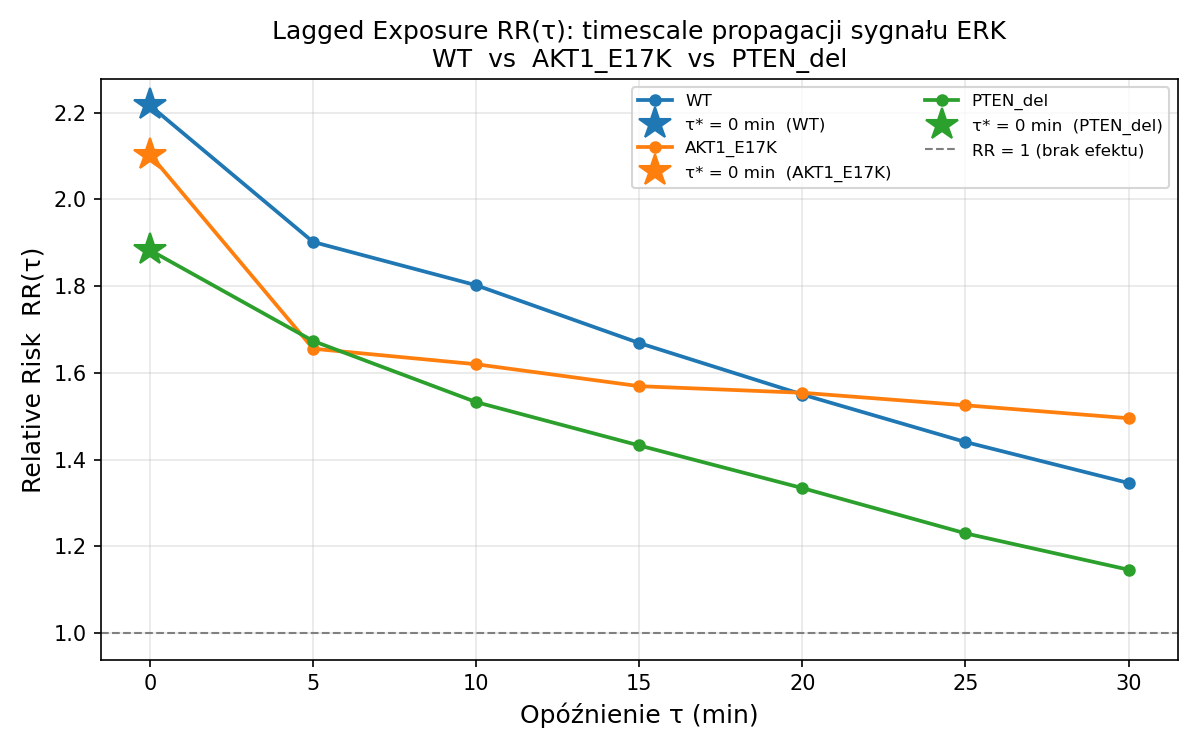
\includegraphics[width=0.82\textwidth]{A2_lagged_RR.png}
  \caption{Lagged Exposure $\mathrm{RR}(\tau)$ vs.\ lag $\tau$ (min) for WT
    (blue), AKT1\_E17K (orange), and PTEN\_del (green).
    Stars mark $\tau^*$; dashed line: $\mathrm{RR}=1$.}
  \label{fig:rr_curves}
\end{figure}

\begin{table}[H]
  \centering
  \caption{Optimal lag $\tau^*$ and maximum Relative Risk for each cell line.}
  \label{tab:summary}
  \begin{tabular}{lccc}
    \toprule
    \textbf{Mutation} & \textbf{$\tau^*$ (frames)} & \textbf{$\tau^*$ (min)} & \textbf{max RR} \\
    \midrule
    WT         & 0 & 0 & 2.216 \\
    AKT1\_E17K & 0 & 0 & 2.103 \\
    PTEN\_del  & 0 & 0 & 1.883 \\
    \bottomrule
  \end{tabular}
\end{table}

\subsubsection{Interpretation}

The lagged exposure analysis reveals that for all three genotypes the maximum
Relative Risk occurs at $\tau^* = 0$ frames (0\,min): WT achieves
$\mathrm{RR}(0) = 2.22$, AKT1\_E17K reaches $\mathrm{RR}(0) = 2.10$, and
PTEN\_del attains $\mathrm{RR}(0) = 1.88$.
The absence of a detectable positive lag is consistent with two scenarios that
cannot be distinguished at the available temporal resolution of 5\,min/frame:
either ERK signal propagation between neighbours occurs on a sub-5-minute
timescale, or neighbouring cells respond nearly simultaneously to a shared
paracrine stimulus rather than relaying the signal sequentially.
In all three genotypes $\mathrm{RR}(\tau)$ decreases monotonically with
increasing lag, confirming that spatial coordination of ERK jumps is a short-lived
phenomenon.

A clear gradient in the magnitude of $\mathrm{RR}(0)$ is observed:
WT $>$ AKT1\_E17K $>$ PTEN\_del.
Oncogenic mutations hyperactivating the PI3K--AKT axis therefore reduce, rather
than amplify, the spatial coordination of ERK jumps.
A plausible explanation is that constitutive AKT activity elevates the rate of
autonomous ERK jumps independent of neighbour signalling, increasing the baseline
jump rate in unexposed cells and diluting the relative contribution of
neighbour-driven activation.
PTEN\_del, acting upstream of AKT through chronic PIP3 elevation, produces the
strongest tonic activation and hence the largest autonomous noise, yielding the
lowest $\mathrm{RR}$.
In summary, whereas $\tau^* = 0$ for all lines precludes distinguishing
propagation timescales at this frame rate, the analysis uncovers a biologically
meaningful difference in the \emph{strength} of spatial coordination: oncogenic
PI3K--AKT mutations attenuate the synchronised propagation of ERK activation waves
across the cell population.

% =============================================================================
\subsection{Task A3}

\end{document}
